\documentclass[journal]{IEEEtran}
\usepackage[a5paper, margin=10mm]{geometry}
%\usepackage{lmodern} % Ensure lmodern is loaded for pdflatex
\usepackage{tfrupee} % Include tfrupee package


\setlength{\headheight}{1cm} % Set the height of the header box
\setlength{\headsep}{0mm}     % Set the distance between the header box and the top of the text


%\usepackage[a5paper, top=10mm, bottom=10mm, left=10mm, right=10mm]{geometry}

%
\setlength{\intextsep}{10pt} % Space between text and floats

\makeindex


\usepackage{cite}
\usepackage{amsmath,amssymb,amsfonts,amsthm}
\usepackage{algorithmic}
\usepackage{graphicx}
\usepackage{textcomp}
\usepackage{xcolor}
\usepackage{txfonts}
\usepackage{listings}
\usepackage{enumitem}
\usepackage{mathtools}
\usepackage{gensymb}
\usepackage{comment}
\usepackage[breaklinks=true]{hyperref}
\usepackage{tkz-euclide} 
\usepackage{listings}
\usepackage{multicol}
\usepackage{xparse}
\usepackage{gvv}
%\def\inputGnumericTable{}                                 
\usepackage[latin1]{inputenc}                                
\usepackage{color}                                            
\usepackage{array}                                            
\usepackage{longtable}                                       
\usepackage{calc}                                             
\usepackage{multirow}                                         
\usepackage{hhline}                                           
\usepackage{ifthen}                                               
\usepackage{lscape}
\usepackage{tabularx}
\usepackage{array}
\usepackage{float}
\usepackage{ar}
\usepackage[version=4]{mhchem}


\newtheorem{theorem}{Theorem}[section]
\newtheorem{problem}{Problem}
\newtheorem{proposition}{Proposition}[section]
\newtheorem{lemma}{Lemma}[section]
\newtheorem{corollary}[theorem]{Corollary}
\newtheorem{example}{Example}[section]
\newtheorem{definition}[problem]{Definition}
\newcommand{\BEQA}{\begin{eqnarray}}
\newcommand{\EEQA}{\end{eqnarray}}

\theoremstyle{remark}


\begin{document}
\bibliographystyle{IEEEtran}
\onecolumn

\title{7.4.34}
\author{INDHIRESH S- EE25BTECH11027}
\maketitle


\renewcommand{\thefigure}{\theenumi}
\renewcommand{\thetable}{\theenumi}

\textbf{Question}. Find the equation of the circle whose radius is 5 and which touches the circle $x^2 +y^2 - 2x - 4y - 20 = 0$ at the point $(5, 5)$.\\
\textbf{Solution}:\\
Let us solve the given equation theoretically and then verify the solution computationally. \\
The general circle equation can be given as:
\begin{align}
  \norm{\Vec{x}}^2+2\Vec{u^T}\Vec{x}+f=0
\end{align}
Let the equation of the first circle be

\begin{align}
  \norm{\Vec{x}}^2+2\Vec{u_1^T}\Vec{x}+f_1=0
\end{align}
The equation of the second circle be:
\begin{align}
    \norm{\Vec{x}}^2+2\Vec{u_2^T}\Vec{x}+f_2=0
\end{align}
From the given information:
\begin{align}
   \Vec{u_1}=\myvec{-1\\-2}\;\;and\;\;f_1=-20
\end{align}
Let $\Vec{c_1}$ and $\Vec{c_2}$ be the centre of the circle 1 and circle 2:
\begin{align}
  \Vec{c_1}=\Vec{-u_1}=\myvec{1\\2}
\end{align}
And also
\begin{align}
   f_1=\norm{\Vec{u_1}}^2-r_1
\end{align}

\begin{align}
  r_1=5
\end{align}
Let P be the point of contact
\begin{align}
    \Vec{P}=\myvec{5\\5}
\end{align}
If the two circle touch each other externally at $\Vec{P}$. So the $\Vec{P},\Vec{c_1}$ and $\Vec{c_2}$ will be collinear and $\Vec{P}$ will divide the points $\Vec{c_1}$ and $\Vec{c_2}$ in the ratio $\frac{r_1}{r_2}:1$
\begin{align}
   \frac{r_1}{r_2}=1
\end{align}
\begin{align}
   \Vec{P}=\frac{\Vec{c_1}+\Vec{c_2}}{2}
\end{align}
\begin{align}
    \myvec{5\\5}=\frac{\myvec{1\\2}+\Vec{c_2}}{2}
\end{align}
\begin{align}
\Vec{c_2}=\myvec{9\\8}
  \end{align}
If two circles touch each other internally we get:

\begin{align}
 \Vec{c_2}=\myvec{1\\2}
\end{align}
This is the same as circle 1, so the two circles touch each other externally.\\
Now
\begin{align}
    r_2=5\;\;and\;\;\Vec{c_2}=\myvec{9\\8}
\end{align}
\begin{align}
\Vec{u_2}=\Vec{-c_2}=\myvec{-9\\-8}
\end{align}

\begin{align}
    f_2=\norm{\Vec{u_2}}^2-r_2
\end{align}
\begin{align}
   f_2=120
\end{align}
Now the required equation of circle is
\begin{align}
   \norm{\Vec{x}}^2+2\Vec{u_2^T}\Vec{x}+f_2=0
\end{align}
\begin{align}
    \norm{\Vec{x}}^2+2\myvec{-9\\-8}^T\Vec{x}+120=0
\end{align}



From the figure it is clearly verified that the theoretical solution matches with the computational solution.\\
\begin{figure}[h]
    \centering
    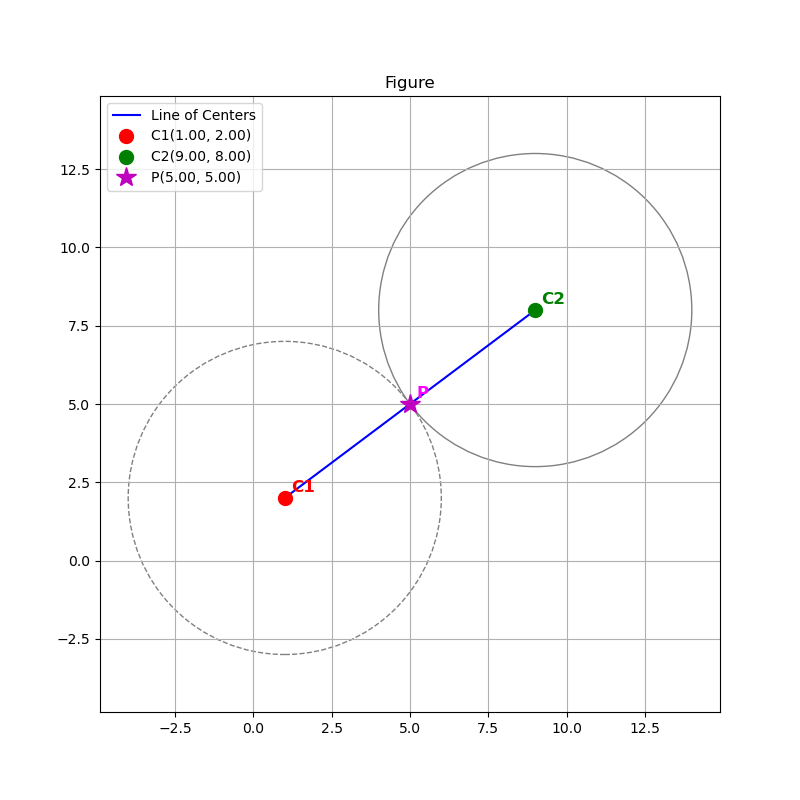
\includegraphics[height=0.5\textheight, keepaspectratio]{figs/figure1.png}
    \label{figure_1}
\end{figure}

\end{document}